\section{Approaches}

\subsection{Community Detection Methods in Network Analysis: Agglomerative and Divisive Approaches}
Community detection in network analysis is a crucial task known as community analytics. It involves identifying groups or communities within a network structure. There are two primary types of community detection methods: agglomerative methods and divisive methods.
\begin{center}
    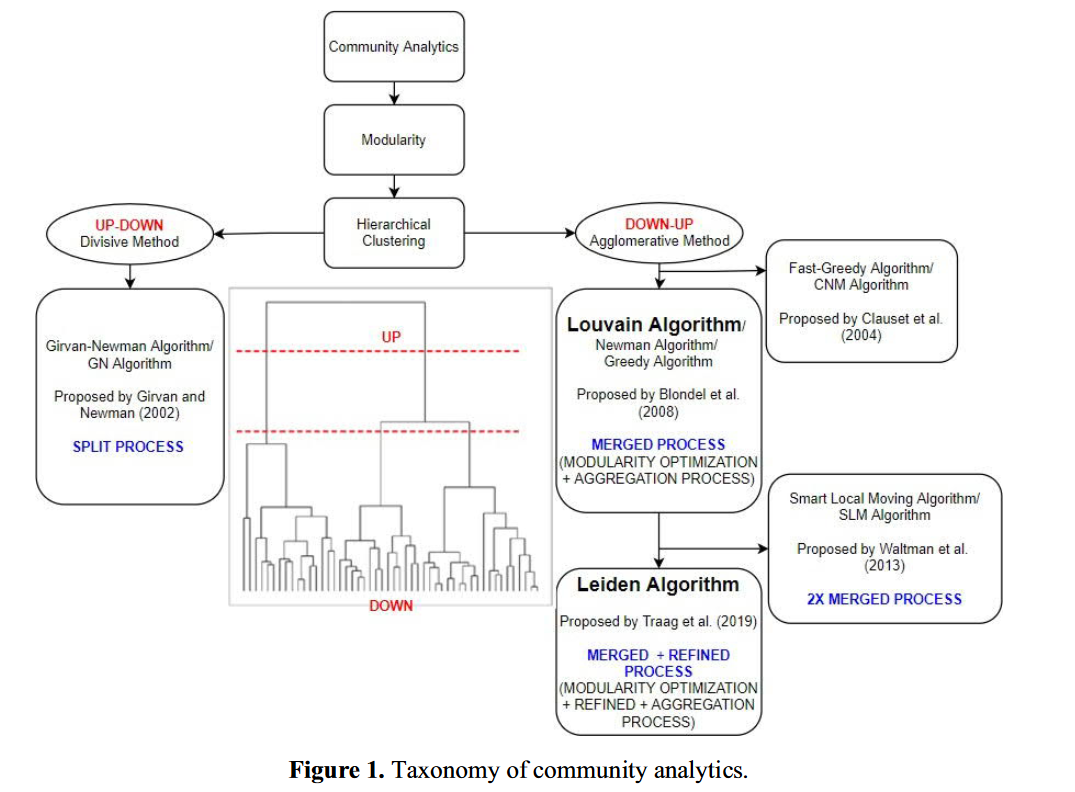
\includegraphics[scale=0.45]{image/jpcsj.png}
\end{center}
In agglomerative methods (shown in the right wing of Figure 1), the process starts from individual nodes and progressively merges them based on their similarity or connectivity, resulting in a hierarchical clustering. This means that nodes are merged from the bottom up, creating larger communities as the process continues. The Louvain and Leiden algorithms, which are based on modularity and hierarchical clustering, fall into the agglomerative category. Modularity, denoted as Q, measures the strength of communities and guides the algorithm. Higher values of modularity indicate better communities, and a value below 1 suggests that each node is considered a separate community. The dendrogram in Figure 1 represents the hierarchy of clusters generated by hierarchical clustering.

On the other hand, divisive methods (depicted in the left wing of Figure 1) start with a single partition containing all nodes and iteratively split it by removing edges with low similarity. This process is known as the split process. Divisive methods aim to find smaller, more cohesive communities by progressively dividing the network.

Both agglomerative and divisive methods have different approaches to community detection, but they ultimately seek to uncover meaningful groups of nodes based on their connectivity patterns within a network.
\subsection{Girvan-Newman algorithm}
The Girvan-Newman algorithm is a well-known community detection algorithm in network analysis. Proposed by Michelle Girvan and Mark Newman, it aims to identify communities or clusters within a network by iteratively removing edges with high betweenness centrality. This algorithm follows a divisive approach, progressively dividing the network into smaller communities based on the importance of edges.\\
\textbf{Edge Betweenness: } It uses edge betweenness to find and remove central edges that connect communities within a larger graph.
The formula for edge betweenness is: \newline
\begin{equation}
    B(e) = \sum_{u,v \in V(G)} \frac{\sigma_{u,v}(e)}{\sigma_{u,v}}
\end{equation}
where $\sigma{_u,v}$ is the number of shortest paths between two distinct vertices and $\sigma_{u,v}(e)$ is the corresponding number of shortest paths containing a particular edge.\\
\textbf{Modularity: } After removing an edge, the Girvan-Newman algorithm calculates the modularity (Q) of the graph, which is a value between the range $[-0.5,1]$. A higher value suggests a more significant community structure. Therefore, we can identify communities by maximizing modularity.\\

The formula for modularity is: 
\begin{equation}
    Q = \sum_{s=1}_m\Big[\frac{l_s}{L}-\Big(\frac{d_s}{2L}\Big)^2\Big]
\end{equation}
(m = number of modules, ls = the number of edges inside module s, L = the number of edges in the network, dₛ = total degree of the nodes in module s)\\

This process of removing an edge and calculating the modularity is iteratively repeated. The algorithm will stop when the new modularity is no longer greater than the modularity from the previous iteration. The ending modularity is usually around 0.6.

\subsubsection{Pseudo Code}
\begin{algorithm}
        \SetAlgoLined
    \SetKwInOut{Input}{Input}
    \SetKwInOut{Output}{Output}
    \SetKwRepeat{Do}{do}{while}

    \Input{Graph $G$}
    \Output{Disconnected components of $G$}

    \BlankLine

    \Do{number of edges in $G$ is not 0}{
        Let $n$ be the number of edges in $G$\;
        
        \For{$i = 0$ to $n-1$}{
            Let $B[i]$ be betweenness centrality of edge $i$\;

            \If{$B[i] > {max_B}$}{
                ${max_B} \gets B[i]$\;
                
                $max_{B(edge)} \gets i$\;
            }

            Remove edge $i$ from graph
        }
    }

    \caption{Girvan-Newman Algorithm}
\end{algorithm}

\subsubsection{Implement Code}
\begin{lstlisting}[language=Python]
def girvan_newman_algorithm(G):
    # calculate initial betweenness centrality of all edges
    betweenness = nx.edge_betweenness_centrality(G)

    while len(G.edges()) > 0:
        # remove edge with highest betweenness centrality
        max_edge = max(betweenness, key=betweenness.get)
        G.remove_edge(*max_edge)

        # recalculate betweenness centrality of remaining edges
        betweenness = nx.edge_betweenness_centrality(G)

        # check if the graph has been split into disconnected components
        if nx.number_connected_components(G) > 12:
            # if so, return the list of communities
            communities = list(nx.connected_components(G))
            return communities

    # if no disconnected components are found, return the original graph as a single community
    return [set(G.nodes())]

\end{lstlisting}

\subsubsection{Pros, Cons}
The Girvan-Newman algorithm offers several advantages and disadvantages in community detection within network analysis.

On the positive side, the algorithm is effective in uncovering the community structure of a network. By targeting edges with high betweenness centrality and iteratively removing them, it reveals the underlying modular organization of the network. This capability allows for a comprehensive understanding of how communities are formed and interconnected.

Additionally, the Girvan-Newman algorithm does not require any prior information or assumptions about the network's structure or the number of communities. It dynamically adapts to the unique characteristics of the network during the divisive process, making it versatile and applicable in various scenarios.

The algorithm also provides valuable insights into bridge edges, which are edges with high betweenness centrality that act as connections between different communities. By identifying these bridge edges, researchers can gain a deeper understanding of the interconnections and relationships between communities.

However, there are also some drawbacks to consider. One major limitation is the computational expense associated with the Girvan-Newman algorithm, especially for large networks. Calculating betweenness centrality for all edges in the network requires significant computational resources, making it impractical for networks with millions of nodes.

Another limitation is the resolution limit of the algorithm. It may struggle to detect smaller communities or communities with weaker connectivity. In some cases, the algorithm tends to merge smaller communities into larger ones, resulting in the loss of fine-grained community structure.

Additionally, the Girvan-Newman algorithm lacks scalability for very large networks. As the network size increases, the algorithm's runtime and memory requirements grow significantly, posing challenges in analyzing massive datasets.

Despite these limitations, the Girvan-Newman algorithm remains a valuable tool for community detection, providing insights into the modular organization of networks. Researchers continue to explore enhancements and alternative approaches to address its drawbacks and improve its applicability in different network analysis scenarios.

\subsubsection{Time Complexity}
Despite Girvan-Newman’s popularity and quality of community detection, it has a high time complexity, increasing up to $O(m^2n)$ on a sparse graph having m edges and n nodes. As a result, Girvan-Newman is generally not used on large scale networks. Its optimal node count is a few thousand nodes or less.

Because of this, there exist greedy algorithms for detecting communities to reduce the time but at the same time sacrificing the most accurate results. One such example is the Louvain algorithm.
\subsection{Louvain Algorithm}
The Louvain algorithm is a fast implementation of community detection. It can be used to analyze a network of 2 million nodes in only 2 minutes \\
\newline
It is a hierarchical clustering algorithm that involves two phases: modularity optimization and community aggregation 
\begin{center}
    \begin{figure}[!htp]
    \centering
    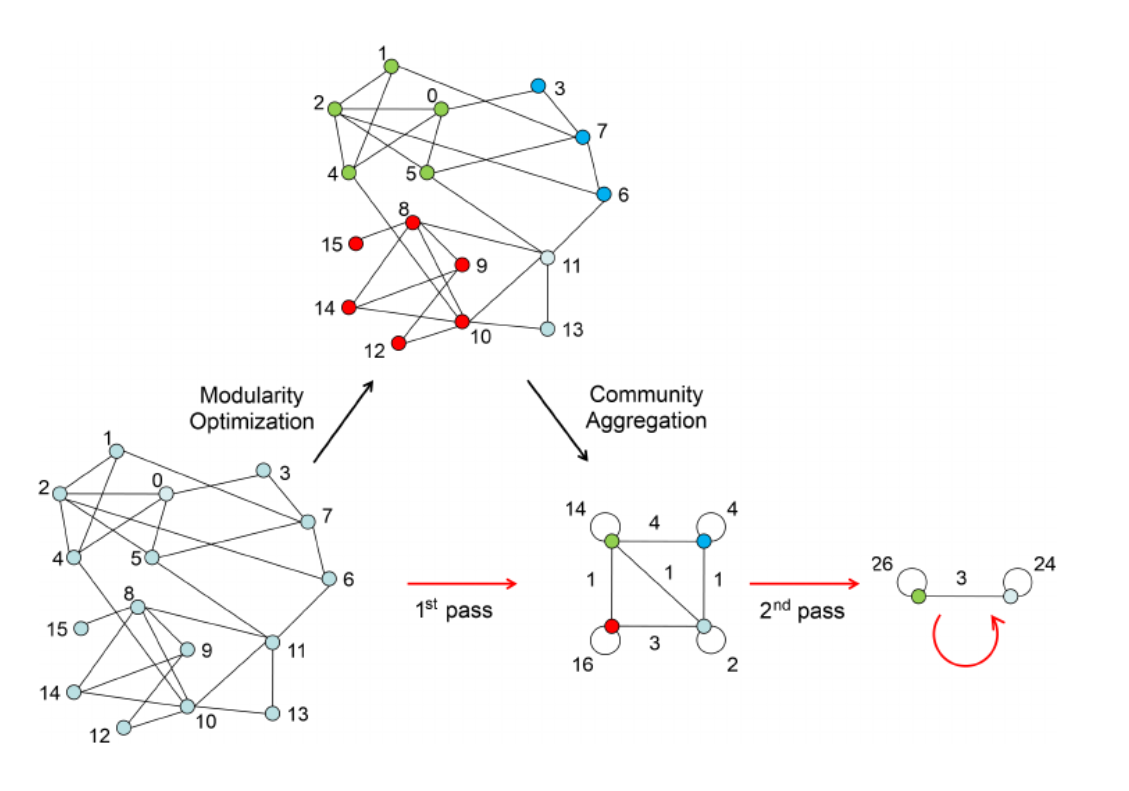
\includegraphics[width=0.7 \textwidth]{image/Louvain.png}
    \caption{Louvain Algorithm}
    \label{subsection}
\end{figure}
\end{center}
\subsubsection{Modularity Optimization}
As seen in the figure, the first step is to optimize the modularity of the entire graph. In this example, it splits the nodes into four communities.

To find these clusters, each node is moved into its neighboring community. If the change in modularity ($\Delta Q$) is greater than 0, it is moved into the neighboring community, Otherwise, it remains in its current community. This process is repeated until $\Delta Q=0$ for all nodes.
\subsubsection{Community Aggregation}
After modularity optimization, super nodes are created to represent each cluster. After the initial phase of the algorithm, there will exist many communities.

However, the two phases repeat, creating larger and larger communities. The algorithm stops only when no improvement can be made by any of the two operations 
\subsubsection{Pros, Cons}
Pros of the Louvain algorithm:
\begin{itemize}
    \item Fast and scalable for large networks.
    \item Optimizes modularity, which measures community quality.
    \item Detects hierarchical community structures.
    \item Allows flexibility in resolution for different levels of detail.
    \item Widely used with extensive resources and documentation.
\end{itemize}

Cons of the Louvain algorithm:
\begin{itemize}
    \item Resolution limit may merge small communities into larger ones.
    \item Results can be sensitive to initial community assignments.
    \item Assumes non-overlapping communities.
    \item Bias towards detecting large, cohesive communities.
    \item Lacks theoretical guarantees of optimality.
\end{itemize}

We need to keep in mind these points when considering the Louvain algorithm for community detection.

\subsubsection{Pseudo Code}
\begin{algorithm}[H]
    \setcounter{AlgoLine}{0}
    \SetAlgoLined
    \SetKwInOut{Input}{Input}
    \SetKwInOut{Output}{Output}

    \Input{Graph $G$}
    \Output{Communities}

    \BlankLine

    Initialize each node in $G$ as a separate community\;
    
    Initialize the change indicator $modularity_{improvement}$\;

    \Repeat{$\text{modularity\_improvement}$ is not positive}{
        $\text{modularity\_improvement} \gets 0$\;

        \For{each node $i$ in $G$}{
            \For{each neighbor $j$ of node $i$}{
                Merge community of node $i$ with community of node $j$\;
                
                Compute the modularity improvement\;
                
                Undo the merge if the improvement is not positive\;
                
                Track the maximum improvement\;
            }
        }
    }

    \caption{Louvain Algorithm}
\end{algorithm}

\subsubsection{Implement Code}
\begin{lstlisting}[language=Python]

def initialize_communities(graph):
    """
    Initialize each node into its own community.
    """
    return {node: [node] for node in graph.nodes()}


def calculate_modularity(graph, communities, m):
    """
    Calculate the modularity of the graph given the communities.
    """
    Q = 0.0
    for community in communities.values():
        community_subgraph = graph.subgraph(community)
        L_c = sum(dict(community_subgraph.degree(weight='weight')).values())
        d_c = 2 * L_c / m
        Q += (L_c / m) - np.square(d_c)
    return Q


def louvain(graph):
    """
    Perform community detection using the Louvain algorithm.
    """
    m = sum(dict(graph.degree(weight='weight')).values()) / 2

    # Step 1: Create initial communities
    communities = initialize_communities(graph)

    # Track the best modularity
    best_modularity = calculate_modularity(graph, communities, m)

    while True:
        # Step 2: Move nodes between communities
        moved = False

        for node in graph.nodes():
            # Get the current community of the node
            current_community = None
            for c, nodes in communities.items():
                if node in nodes:
                    current_community = c
                    break

            # Calculate the modularity gain of moving the node to each neighboring community
            neighbor_communities = set()
            for neighbor in graph.neighbors(node):
                for c, nodes in communities.items():
                    if neighbor in nodes:
                        neighbor_communities.add(c)

            modularity_gains = {}
            for neighbor_community in neighbor_communities:
                communities[current_community].remove(node)
                communities[neighbor_community].append(node)

                modularity_gains[neighbor_community] = calculate_modularity(graph, communities, m)

                # Move the node to the community with the maximum modularity gain
                max_gain_community = max(modularity_gains, key=modularity_gains.get)
                max_gain = modularity_gains[max_gain_community]

                if max_gain > 0:
                    communities[max_gain_community].append(node)
                    moved = True
                    break

                # If no improvement, revert the move
                communities[neighbor_community].remove(node)
                communities[current_community].append(node)

        # If no nodes have moved communities, stop iterating
        if not moved:
            break

        # Recalculate modularity
        modularity = calculate_modularity(graph, communities, m)

        # If modularity has improved, update the best modularity
        if modularity > best_modularity:
            best_modularity = modularity

    return communities.values()
\end{lstlisting}

\subsection{Leiden algorithm}
% \subsubsection{Introduction}
The Leiden algorithm is an algorithm for detecting communities in large networks. It separates nodes into disjoint communities so as to maximize a modularity score for each community. Modularity quantifies the quality of an assignment of nodes to communities, that is how densely connected nodes in a community are, compared to how connected they would be in a random network. The Leiden algorithm extends the Louvain algorithm, which is widely seen as one of the best algorithms for detecting communities. However, the Louvain algorithm can lead to arbitrarily badly connected communities, whereas the Leiden algorithm guarantees communities are well-connected.\\
This algorithm is processed included 3 step:\\
\begin{itemize}
    \item Step 1: local moving of nodes.
    \item Step 2: Refinement of the partition.
    \item Step 3: Aggregation of the network based on the refined partition.
\end{itemize}
We can see this process in the picture from (a) to (f) as below. It starts from a singleton partition (a). The algorithm moves individual nodes from one community to another to find a partition (b), which is then refined (c). An aggregate network (d) is created based on the refined partition, using the non-refined partition to create an initial partition for the aggregate network. For example, the red community in (b) is refined into two subcommunities in (c), which after aggregation become two separate nodes in (d), both belonging to the same community. The algorithm then moves individual nodes in the aggregate network (e). In this case, refinement does not change the partition (f). These steps are repeated until no further improvements can be made.
\begin{figure}[H]
    \centering
    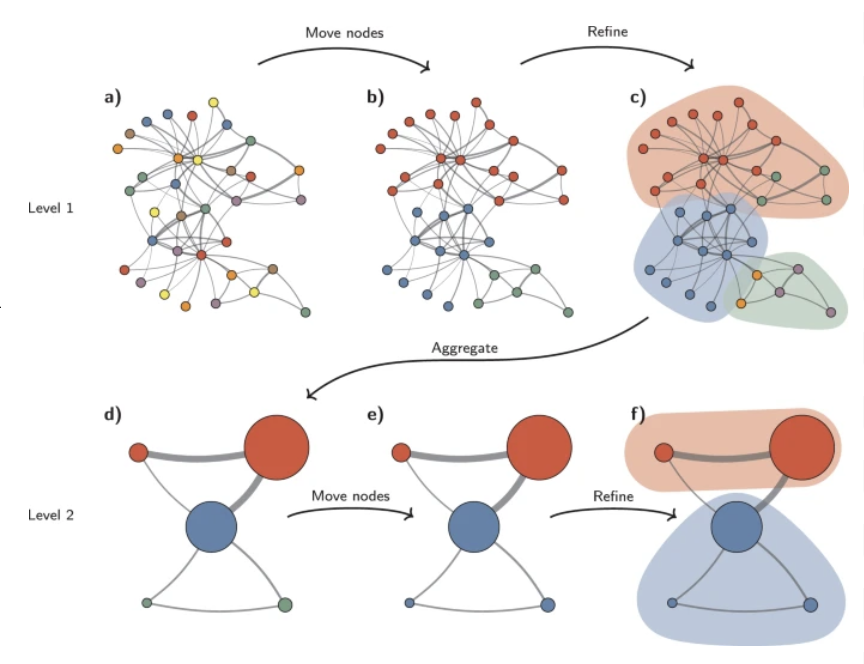
\includegraphics[width=12cm]{image/6.png}
    \caption{The Leiden algorithm}
\end{figure}
\subsubsection{Pseudo code}
\begin{figure}[H]
    \centering
    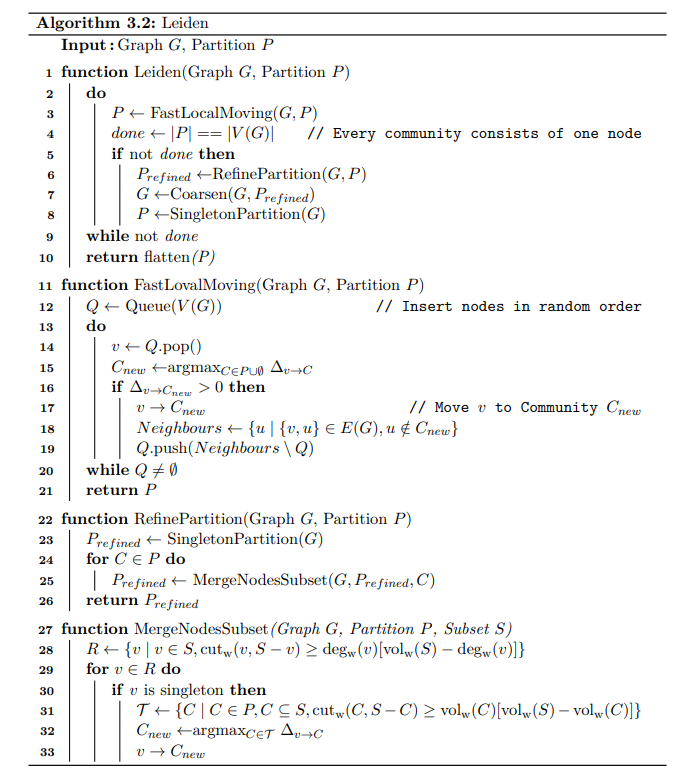
\includegraphics[width=1\textwidth]{image/pseudo code.png}
  
\end{figure}

\subsubsection{Pros, Cons}
The Leiden algorithm is a popular community detection algorithm that has been used in various fields, including social network analysis and bioinformatics. Some of the advantages of the Leiden algorithm are:
\begin{itemize}
    \item It is a fast and scalable algorithm that can handle large and complex networks.
    \item It can detect communities of different sizes and densities.
    \item It can handle directed and weighted networks.
    \item It has been shown to perform well in comparison to other community detection algorithms.
\end{itemize}
However, there are also some potential limitations and drawbacks of the Leiden algorithm, such as:
\begin{itemize}
    \item It may not be suitable for detecting communities with overlapping nodes.
    \item It may not perform as well in networks with low modularity.
    \item It may be sensitive to the choice of resolution parameter.
    \item It may require some expertise in parameter tuning and interpretation of results.
\end{itemize}
